\section{Reducing the MPI grid setup and initial load balancing overhead}


\chapterDescription
  {
    Around 30 minutes.
  }
  {
    A working MPI code.
  }


In this section, we assume that you've a reasonable load balancing and that you
were able to postprocess your performance analysis outputs. We discuss issues
that arise over and over again for parallel applications.


\subsection{Massive grid on rank 0 with long redistribution phase
afterwards}

\begin{center}
  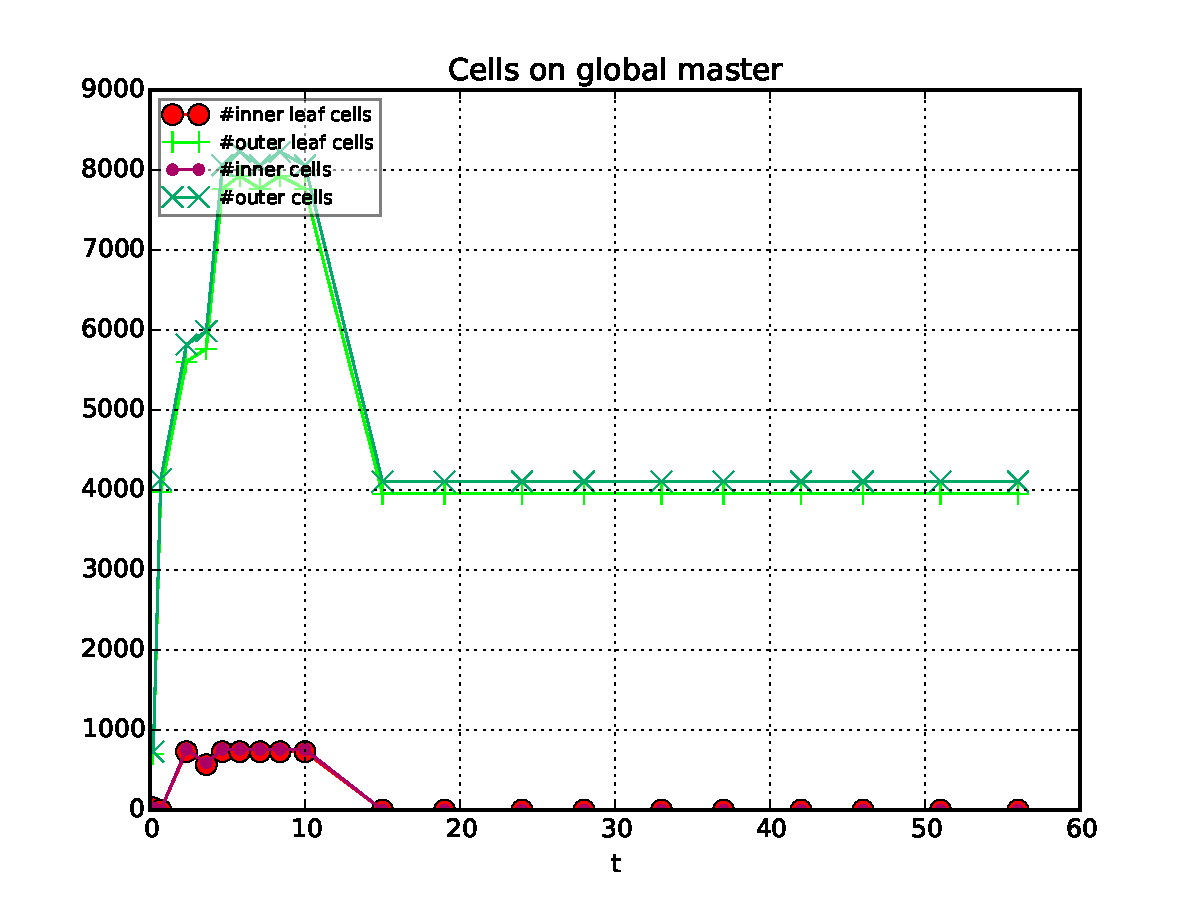
\includegraphics[width=0.5\textwidth]{61_mpi-setup/performance-analysis-output.pdf}
\end{center}


\begin{smell}
There are ranks (notably rank 0) that are assigned lots of cells and vertices
and then this number decreases though the grid should be more or less static.
\end{smell}

\noindent
We observe this behaviour either through a performance analysis (see plot above)
or by outputs from the state where the grid depth immediately goes up to the
maximum depth while the load balancing still splits up things. 
The iterations already are very expensive; obviously as the grid is already in
place but the ranks are not all employed.


The reason for this behaviour can be found in the semantics of
\texttt{createVertex} and \linebreak
\texttt{touchVertexFirstTime}.
Both operations try to refine the grid around the respective vertex immediately. 
Only if circumstances such as a parallel partitioning running through this
vertex---the refinement instruction then first has be distributed to all ranks
holding a copy of this vertex---do not allow Peano to realise the refinement
immediately, the refinement is postponed to the next iteration.
In many parallel codes, all the refinement calls pass through immediately on
rank 0 before it can spawn any rank.
This leads to the situation that the whole grid is in one sweep built up on the
global master and afterwards successively distributed among the ranks.


Such a behaviour is problematic: the global rank might run out of memory, lots
of data is transferred, and the sweeps over the whole grid on rank 0 are
typically pretty expensive. 
A distributed grid setup is advantageous.

\begin{solution}
Switch from an aggressive
refinement into an iterative grid refinement strategy to allow the ranks to
deploy work throughout the grid construction and thus build up the grid in parallel and avoid the transfer of whole grid
blocks due to rebalancing.
\end{solution}

\noindent
The simplest materialisation of this idea is to 
move your \texttt{refine()} calls from the creational or touch first
events into \texttt{touchVertexLastTime()}:
As a consequence, setting up a (rather regular) grid of depth $k$ requires at
least $k$ iterations.

This still might be insufficient---it depends strongly on the type of load
balancing you use; some need several iterations to determine proper rebalancing
while even your incremental grid construction might already have run into very
fine grids---so I found it useful to augment the state such that my global
master can instruct all ranks whether they are allowed to refine or not. 
Permission is then granted only from time to time.


\begin{remark}
 I present a sophisticated yet very simple grid construction pattern not
 replicating any refinement code throughout Section
 \ref{subsection:mpi-setup:slow-incremental-setup}.
\end{remark}

% In a second step, you might consider to extend your grid only every second
% traversal.
% Everytime you rebalance your grid, Peano disables dynamic load balancing
% for a couple of iterations (three or four). Throughout these iterations, it
% can recover all adjacency information if the grid itself changes as well.
% Consequently, it does make sense to add a couple of adapter runs after each
% grid modification that to not change the grid structure: When you know that
% you have an adapter that changes the grid, apply afterwards an adapter that
% does not change the grid for a couple of times. This way, you ensure that no
% mpi rank runs out of memory. The grid generation does not overtake the rebalancing.
% I often do not use an additional adapter but ensure that refines are only called
% if the tree traversal direction is not inverted: 
% Peano runs forth and back through the grid, so this effectively switches off
% refinement every second iteration. 
% 
% The deluxe version is a code that refines only if the previous grid traversal
% did not change the mesh, if no load balancing is going anymore and, for example,
% \texttt{isTraversalInverted()} does not hold. This postpones any refinement
% further.
% However, such an approach is a bad idea if no idle nodes are available anymore. 
% In this case, it is better not to veto the refinement anymore.
% This situation is discussed in the following bad smell, where we propose a
% sophisticated solution to both smells.



\subsection{Incremental, slow decomposition with ranks running out
of memory}
\label{subsection:mpi-setup:slow-incremental-setup}


\begin{smell}
Peano needs lots of iterations to finally build the grid up and distribute it
properly.
Often, some ranks run out of memory if the grid is reasonably fine.
\end{smell}



\noindent
The smell is notably cumbersome if the kernel continues to ``balance'' and
incremental build up the grid though all ranks are already busy.
And it is annoying that ranks tend to run out of memory at the same
time---the load balancing cannot keep pace with the grid construction.
In the following, we first give an explanation for this behaviour, we then
sketch the tools offered by Peano to ``cure'' it, and then we sketch an overall
code design/pattern to overcome the smell.


Peano exchanges the vertices along a domain boundary after each traversal.
At the same time, it tries to refine a vertex with a refinement flag as soon as
possible: 
if a code sets a refine command upon creation of a vertex or when a vertex is
loaded for the very first time, it immediately refined.
If refine is called later throughout the traversal, Peano has to memorise the 
refinement request and wait for the subsequent traversal as all adjacent cells
have to anticipate an ongoing refinement but some have already been processed.
To ensure that the grid is always consistent, vertices at a domain boundary
never can be refined immediately. 
These guys are exchanged after each traversal and merged with their counterpart
on other ranks prior to the next usage. 
Refinement triggers thus never are available immediately on other ranks---these
vertices are replicated not held synchronous.

This behaviour implies that the grid can be built up at most by one level per
iteration along domain boundaries.
Therefore, we often see codes running many iterations until a  grid is
built up completely.
Often, this is not necessary as all ranks would know without any data
exchange where to refine (a certain mesh size might be prescribed, e.g.).
For this case, Peano provides a function \texttt{enforceRefine} in the parallel
mode that tells the code not to bother about data consistency and to refine 
everywhere. 
Basically, the user tells the grid that he accepts responsibility to call 
\texttt{enforceRefine} on all replicants of a vertex.
We may not use the enforced refinement if we still want Peano to load
balance/split the grid; if we used the enforce, our strategy would render all
discussions from the previous section useless.


\begin{solution}
Use \texttt{enforceRefine} once no idle ranks are left anymore for all grid
refinement where all ranks know a priori that they have to refine.
\end{solution}


We have to be very careful to use the enforced refinement.
We may use it if and only if there are no more idle nodes available and if all
previous forks and joins have successfully passed through. 
This is information that is available only on the global master. 

%\begin{remark}
A working and simple grid setup pattern is described as follows:
\begin{enumerate}
  \item We add a field
    \begin{code}
      persistent parallelise int maxRefinementLevelAllowed;
    \end{code}
    to the \texttt{State.def} it will keep track to which degree any rank is
    allowed to refine the grid. 
    The semantics of this field are as follows:
    \begin{center}
     \begin{tabular}{lp{12cm}}
       Value & Semantics \\
       \hline
       0 & Initial value \\
         & No refinement is permitted. 
       \\
       \hline
       $>0$ & Whenever we end a sweep where no rebalancing has been made at all
       and the grid hasn't changed in this sweep (is stationary), i.e.~no new
       ranks have entered the game, we increment the counter.
       Refinements are allowed up to the level of
       \texttt{maxRefinementLevelAllowed}. Refinement beyond that are vetoed. 
       \\
       \hline
       -1 & Value is set as soon as there are no idle ranks left anymore. \\
          & Allow standard refinements in both creational and non-creational
          events. \\
          & After the next iteration, reduce \texttt{maxRefinementLevelAllowed}
          to -2.
       \\
       \hline
       $-2$ & We know that no idle workers are left anymore and that another
       sweep has already terminated since the last worker has been given out, i.e.,
       we may assume that all workers now have joined the game and the forks
       have completed (a fork needs two iterations to finish; one to exchange
       administrative/meta data and one to transfer the actual data). From
       hereon, we may safely use the enforced refinement without boundary data
       exchange if we know the adaptivity pattern on each rank.
       \\
       \hline
       $\leq -3$ & This value indicates that we can stop the grid construction,
       as we have constructed the whole thing.
     \end{tabular}
    \end{center}

  \item We augment the state: from hereon, the state can co-decide whether and
    how a mapping refines:
    \begin{code}
    // Has to be called after the iteration!
    void endedGridConstructionIteration(int finestGridLevelPossible);

    enum RefinementAnswer {
      DontRefineYet,
      Refine,
      EnforceRefinement
    };
    RefinementAnswer mayRefine(bool isCreationalEvent, int level) const;

    bool continueToConstructGrid() const;
    \end{code}


  \item We update the state after each grid setup sweep and we delegate the
  decision when to terminate the iterate grid construction to the state.
  Code then might resemble
    \begin{code}
  while ( repository.getState().continueToConstructGrid() ) {
    repository.iterate();
    repository.getState().endedGridConstructionIteration(maxLevel);
  }
    \end{code}
    Note that it is important for the state to know what the maximum grid level
    might be in the end. You may want to use an upper bound that is not too
    inaccurate. This upper bound will kick in if and only if there are more MPI
    ranks than a grid can actually employ.

  \item We restructure the grid creation mapping. Both
    \texttt{createInnerVertex}, \texttt{createBoundaryVertex} and
    \texttt{touchVertexLastTime} now call a routine \texttt{refineIfNecessary}
    that we make accept a boolean that tells it whether it has been invoked by a
    creational event.
    \begin{code}
void ...::mappings::...::refineIfNecessary(
  ...::Vertex&  fineGridVertex,
  ...,
  int           fineGridLevel,
  bool          isCreationalRoutine
) {
  if (
    my code wants to refine
    &&
    fineGridVertex.getRefinementControl()==Vertex::Records::Unrefined
  ) {
    switch ( _state.mayRefine(isCreationalRoutine,fineGridLevel) ) {
      case State::RefinementAnswer::DontRefineYet:
        break;
      case State::RefinementAnswer::Refine:
        fineGridVertex.refine();
        break;
      case State::RefinementAnswer::EnforceRefinement:
        fineGridVertex.enforceRefine();
        break;
    }
  }
}
    \end{code} 
    The routine basically delegates the real refinement decision to the state. 
  \item So, finally, the state has to define whether to refine or not. We
  accomplish this through two routines:
  \begin{code}
void ...::State::endedGridConstructionIteration(int finestGridLevelPossible) {
  const bool idleNodesLeft = 
    tarch::parallel::NodePool::getInstance().getNumberOfIdleNodes()>0;
  const bool nodePoolHasGivenOutRankSizeLastQuery = 
    tarch::parallel::NodePool::getInstance().hasGivenOutRankSizeLastQuery();

  // No more nodes left. Start to enforce refinement
  if ( !idleNodesLeft 
    && _stateData.getMaxRefinementLevelAllowed()>=0 
    && !nodePoolHasGivenOutRankSizeLastQuery) {
    _stateData.setMaxRefinementLevelAllowed(-1);
  }
  // Seems that max permitted level has exceeded max grid level. We may assume
  // that there are more MPI ranks than available trees.
  else if (isGridStationary() 
    && _stateData.getMaxRefinementLevelAllowed()>finestGridLevelPossible
    && _stateData.getMaxRefinementLevelAllowed()>=0 
    && !nodePoolHasGivenOutRankSizeLastQuery) {
    _stateData.setMaxRefinementLevelAllowed( -1 );
  }
  // Reset counter by two. Some LB has happened and we might wanna
  // give the whole system two sweeps to recover from this LB, i.e. to
  // set up all partitions properly and recompute all LB metrics.
  else if (nodePoolHasGivenOutRankSizeLastQuery 
    && _stateData.getMaxRefinementLevelAllowed()>=2) {
    _stateData.setMaxRefinementLevelAllowed(
      _stateData.getMaxRefinementLevelAllowed()-2);
  }
  // Refinement is enforced. So we decrease counter. Once we underrun -2, grid
  // construction can terminate as all enforced refined instructions went
  // through. 
  else if (_stateData.getMaxRefinementLevelAllowed()<=-1  
    && !nodePoolHasGivenOutRankSizeLastQuery 
    && isGridStationary()) {
    _stateData.setMaxRefinementLevelAllowed( 
      _stateData.getMaxRefinementLevelAllowed()-1 );
  } 
  // Nothing has changed in this grid iteration in the grid and we have not
  // given out new workers. So increase the permitted maximum grid level by
  // one and give another try whether the grid adds more vertices.
  else if (
       (!nodePoolHasGivenOutRankSizeLastQuery)
    && isGridStationary()
    && (_stateData.getMaxRefinementLevelAllowed()>=0)
  ) {
    _stateData.setMaxRefinementLevelAllowed(
      _stateData.getMaxRefinementLevelAllowed()+1);
  }
}
  \end{code}
  
  \noindent
  Our \texttt{maxRefinementLevelAllowed} acts as a guardian for the refinement.
  It is updated on the global master after each traversal and then propagates to
  all children. 

  \begin{code}
...::State::RefinementAnswer ...::State::mayRefine(
  bool isCreationalEvent, int level) const 
{ 
  #ifdef Parallel
  if (
    _stateData.getMaxRefinementLevelAllowed()<=-2
    &&
    isCreationalEvent
  ) {
    return RefinementAnswer::EnforceRefinement;
  }
  else if ( _stateData.getMaxRefinementLevelAllowed()<0 ) {
    return RefinementAnswer::Refine;
  }
  else if (
    _stateData.getMaxRefinementLevelAllowed()>level
    &&
    !isCreationalEvent
    &&
    mayForkDueToLoadBalancing()
  ) {
    return RefinementAnswer::Refine;
  }
  else {
    return RefinementAnswer::DontRefineYet;
  }
  #else
  if (isCreationalEvent) {
    return RefinementAnswer::Refine;
  }
  else {
    return RefinementAnswer::DontRefineYet;
  }
  #endif
}
  \end{code}
  
  \noindent
  The serial variant of this routine is straightforward: we refine within the
  creational events. The parallel version makes distinctions depening on
  \texttt{maxRefinementLevelAllowed}.
  There are a few subtle issues here that result from lessons learned:
  Once all nodes are booked, i.e.~no more nodes are idle, we may not immediately
  switch on the enforced refinement. We have to wait one more sweep to allow the
  very last MPI rank that started its work to join the computation completely
  (Peano forks always require two grid sweeps). Therefore, we run the index from
  -1 to -2 before we enable the enforcement. Once a grid becomes stationary and
  no more ranks have joined the game in an iteration, we do not immediately
  increase the maximum refinement level. Instead, we memorise this situation in
  a static bool and then, if the situation hasn't changed, increase the maximum
  refinement level. This way, we allow any load balancing to decide that even on
  the coarser levels there's still some decomposition to be made. Actually, we
  postpone the increase of the level once more: we memorise that we might
  increase the level, and then set the grid to invariant. This way, we enforce
  that the grid does not become balanced which in turn means that the next time
  we run into the routine no forking branch is entered.
  
 \item We stop the grid traversal as soon as the new marker is set to
 -3:
  \begin{code}
bool ...::State::continueToConstructGrid() const {
  #ifdef Parallel
  return _stateData.getMaxRefinementLevelAllowed()>=-3;
  #else
  return !isGridBalanced();
  #endif
}
  \end{code}
  
  \item We finally initialise our state properly:
  \begin{code}
myproject::State::State() : Base() {
  _stateData.setMaxRefinementLevelAllowed(0);
}
  \end{code}
\end{enumerate}
%\end{remark}


%endedGridConstructionIteration

\subsection{The load balancing kicks in immediately while I build up my grid but it
yields non-reasonable partitions}


\begin{smell}
The code runs over the grid a couple of times and starts to distribute the
domain level-by-level as we rely on an incremental build-up. This is however not
clever as it turns out later throughout the grid construction that some regions
are heavily refined while others remain coarse.
\end{smell}


\noindent
If this is the case, it might be reasonable to build up the grid up to a certain
level where grid characteristics become visible, and to switch off the load
balancing while you do so.
Afterwards, load balancing can be enabled and should yield better results. 
Peano allows you to switch off the load balancing, but you have to do this on
each individual rank. 

\begin{code}
peano::parallel::loadbalancing::Oracle::getInstance().activateLoadBalancing(false);
\end{code}


You might want to use
\begin{code}
void myproject::runners::Runner::runGlobalStep() {
  // assertion( !peano::parallel::loadbalancing::Oracle::getInstance().
  // isLoadBalancingActivated() );

  peano::parallel::loadbalancing::Oracle::getInstance().activateLoadBalancing(false);
}
\end{code}

\noindent
to switch off load balancing globally.



\subsection{The load balancing seems not to use all ranks}

\noindent
Peano uses a subscriber pattern to manage all the MPI ranks, while rank 0 is
resopnsible for the actual load/rank assignments.
At startup, rank 0 knows nothing about all the other MPI ranks available.
They have to register at rank 0 (the node pool).
Ranks that want to shared work, ask at the node pool for free ranks and then get
assigned no co-workers.
It thus may happen that a rank asks at the node pool for idle MPI ranks and is
told that no rank is registers though the registration message was just pending
in the queue, i.e.~there would have been further MPI ranks available.
This happens rarely (you then might receive a fork failed notice; depending on
your load balancing), but there is another indicator.

\begin{smell}
  At startup, I receive a lot of messages alike \texttt{node pool does not
  contain entry for rank 3. Message from rank 3 might have overtaken
  registration message. Waiting for registration} if I compile with
  \texttt{-DAsserts}.
\end{smell}

\noindent
A solution to this problem is simple though it (very slightly) increases the
code's startup time.
Please note that it will not make this particular message go away:  
It usually shows up if a rank (here it is rank 3) requests work though its
registration message is still in the queue and hasn't been processed yet.

What you can do is invoke 
\begin{code}
  tarch::parallel::NodePool::getInstance().restart();
  tarch::parallel::NodePool::getInstance().waitForAllNodesToBecomeIdle();
\end{code}
\noindent
just after the restart.
The wait command degenerates to nop if you call it on a rank that is not the
global master, so it is save to call it on every rank.
